% Adaptación de formato: clase y tipografía de la plantilla proporcionada.
% Compilar con: latexmk -pdf -interaction=nonstopmode -halt-on-error main.tex
\documentclass[12pt,spanish,oneside,openany]{MastersDoctoralThesis}
\usepackage[utf8]{inputenc}
\usepackage[T1]{fontenc}
\usepackage{palatino}
\usepackage{amsmath,amssymb}
\usepackage{array,tabularx}
\usepackage{microtype}
\usepackage{listings}
\usepackage{pdfpages}
\onehalfspacing
\decimalpoint
\graphicspath{{figuras/}}
\setlength{\emergencystretch}{2em}
\renewcommand{\thesection}{\arabic{section}}
\renewcommand{\thesubsection}{\thesection.\arabic{subsection}}
\setcounter{tocdepth}{1}
\numberwithin{equation}{section}
\renewcommand{\sectionmark}[1]{\markright{#1}}
\fancypagestyle{thesis}{%
  \fancyhf{}%
  \fancyhead[L]{\small\slshape\nouppercase{\rightmark}}%
  \fancyhead[R]{\small\thepage}%
}
% Completar estos campos con los datos reales del equipo.
\newcommand{\Universidad}{[Universidad]}
\newcommand{\Facultad}{[Facultad]}
\newcommand{\Escuela}{[Escuela profesional]}
\newcommand{\IntegranteUno}{[Nombre y apellidos del integrante 1]}
\newcommand{\IntegranteDos}{[Nombre y apellidos del integrante 2]}
\newcommand{\Docente}{[Nombre y apellidos del docente]}

\thesistitle{Modelo dinámico de la transmisión de dengue humano-mosquito con control vectorial}
\author{\IntegranteUno; \IntegranteDos}
\university{\Universidad}
\faculty{\Facultad}
\department{\Escuela}
\supervisor{\Docente}
\hypersetup{pdftitle={Modelo de dengue: análisis LHS/PRCC},pdfauthor={Equipo de dos integrantes},pdfsubject={Biología Computacional}}
\lstset{basicstyle=\ttfamily\footnotesize,breaklines=true,columns=fullflexible,frame=single,keepspaces=true}
\newcommand{\fuentepropia}{Elaboración propia a partir de las ecuaciones y los resultados de simulación.}
\newcommand{\grafico}[4]{%
\begin{figure}[!htbp]\centering
\includegraphics[width=#2\linewidth]{#1}
\caption{#3}\label{#4}
\end{figure}}
\begin{document}
\frontmatter
\pagestyle{plain}
% Bloque de carátula extraído del PDF original, conservando su posición.
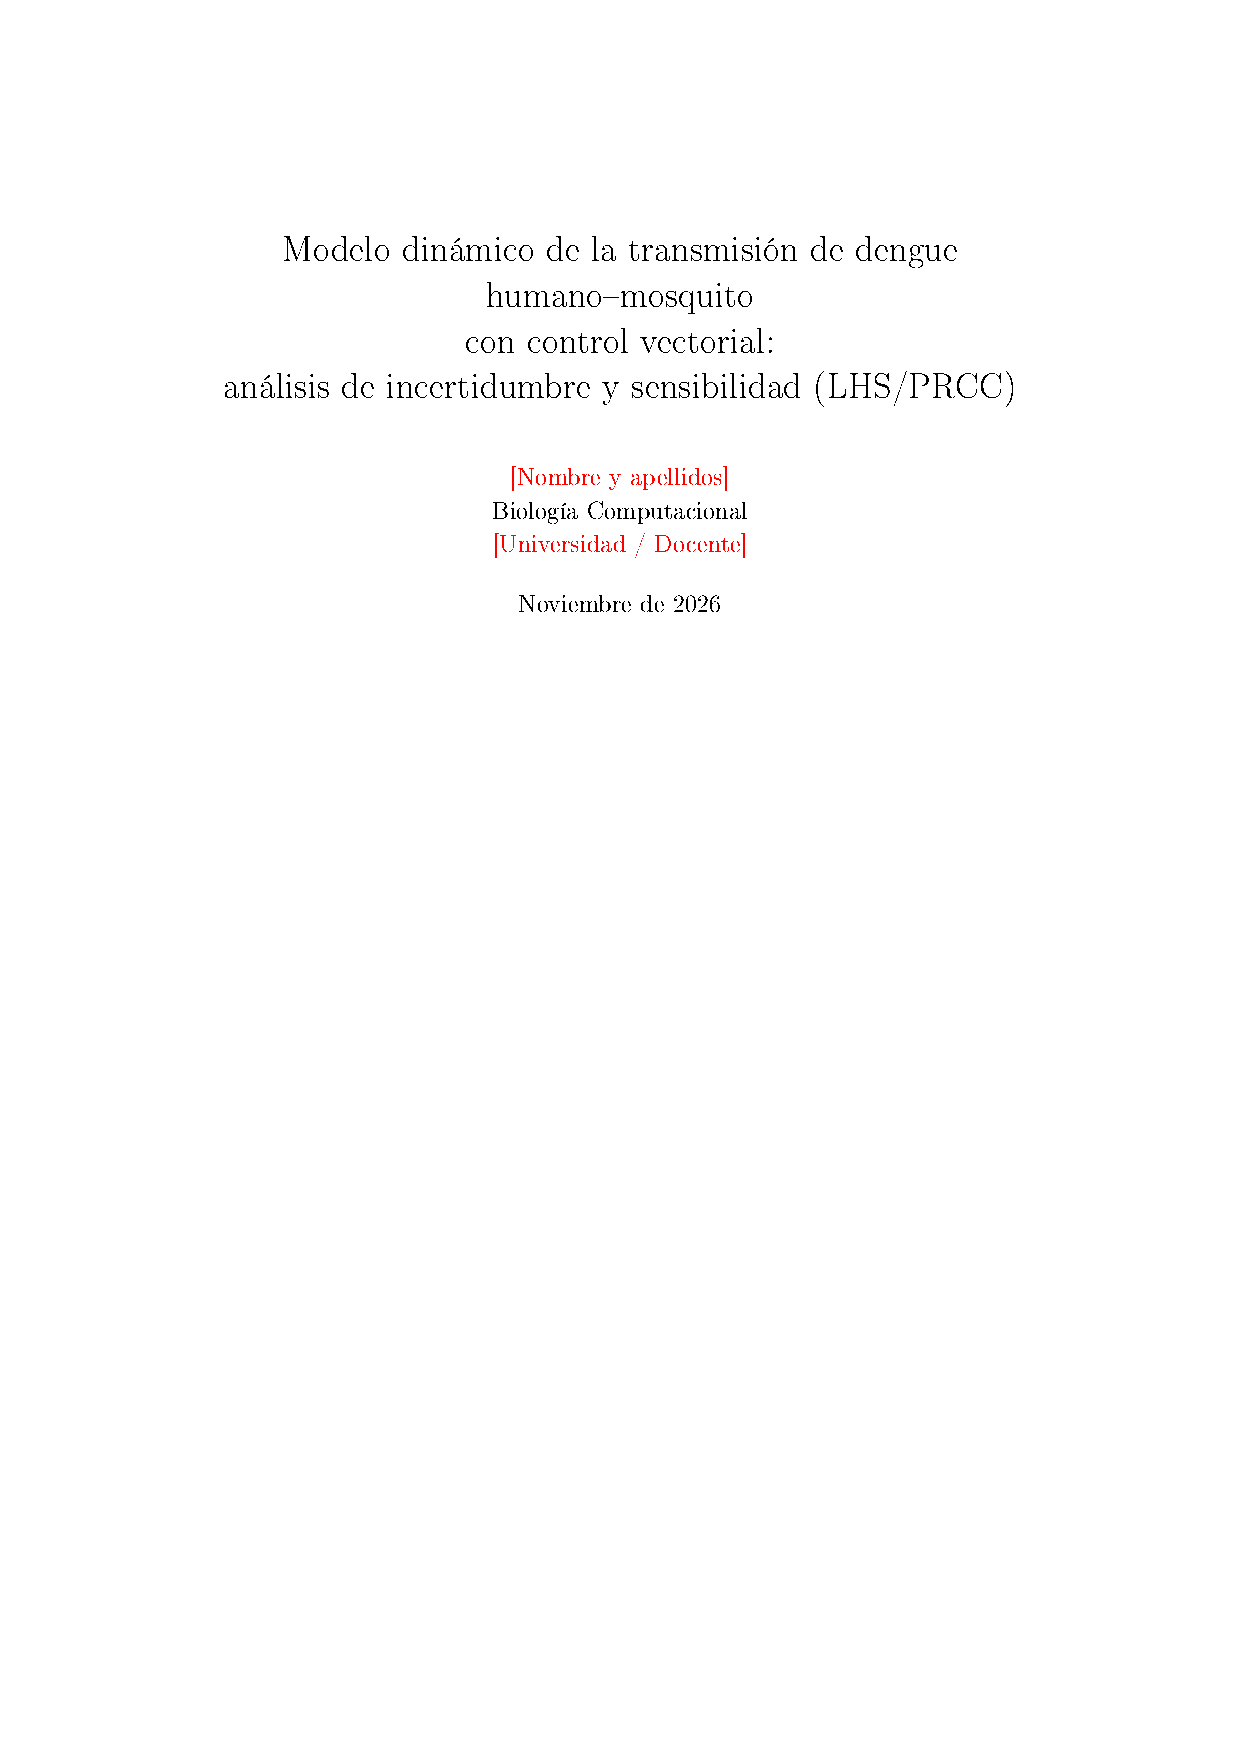
\includepdf[pages=1,pagecommand={\thispagestyle{empty}},fitpaper=true]{figuras/caratula_original.pdf}
\setcounter{page}{1}
\section*{Resumen}
\addcontentsline{toc}{section}{Resumen}
Se estudia la transmisión del dengue mediante un modelo de ecuaciones diferenciales con compartimentos SEIR para humanos y SEI para mosquitos. El control vectorial se representa mediante una mortalidad adicional constante. El sistema se resuelve durante 365 días y se analiza la incertidumbre de nueve parámetros con 999 muestras de hipercubo latino (LHS). La sensibilidad se cuantifica mediante coeficientes de correlación parcial de rangos (PRCC).

Con los parámetros nominales, la prevalencia humana alcanza aproximadamente el 6.65\,\% alrededor del día 112 y el acumulado a 365 días es el 93.36\,\% de la población de referencia. El número reproductivo en el equilibrio con control es aproximadamente 1.82. En el análisis LHS, la tasa de picadura, la probabilidad de transmisión al humano y la densidad vectorial presentan asociaciones positivas con el acumulado. El control vectorial y las tasas de recuperación humana y mortalidad del mosquito presentan asociaciones negativas. Estos resultados describen el comportamiento del modelo dentro de los rangos asumidos; su aplicación a un brote concreto requeriría calibración con datos epidemiológicos.

\clearpage
\tableofcontents
\clearpage
\mainmatter
\pagestyle{thesis}

\section{Problema y objetivo}
El dengue se transmite mediante el contacto entre humanos y mosquitos. La incubación en ambos organismos introduce retardos entre una infección y la posibilidad de transmitirla. Esta interacción permite estudiar cómo las características biológicas del vector y las medidas de control modifican la evolución de una epidemia.

El objetivo es identificar qué parámetros influyen en el acumulado de infecciones, la intensidad del pico y el momento en que ocurre. Se utiliza un modelo SEIR-SEI, con el trabajo de Esteva y Vargas como antecedente de la estructura de transmisión humano-mosquito \cite{esteva}. Las clases de expuestos y la mortalidad adicional por control forman parte de la formulación utilizada en este informe.

El estudio comprende la construcción del modelo causal y dinámico, su solución numérica y un análisis de incertidumbre y sensibilidad. Los parámetros representan escenarios de exploración y no están calibrados con un brote observado.

\section{Modelo causal y dinámico}
\subsection{Variables y relaciones causales}
Los niveles humanos son los susceptibles $S_h$, los expuestos $E_h$, los infecciosos $I_h$ y los recuperados $R_h$. Se expresan como fracciones de una población humana constante. Los niveles vectoriales $S_v$, $E_v$ e $I_v$ corresponden a mosquitos susceptibles, expuestos e infecciosos, expresados respecto de su población basal. La variable $C_h$ cuenta la acumulación de entradas a la clase infecciosa humana desde el inicio de la simulación.

El bucle reforzador de transmisión sigue el recorrido $I_h\to E_v\to I_v\to E_h\to I_h$. Un aumento de humanos infecciosos produce más infecciones del vector; los mosquitos que sobreviven a la incubación transmiten a humanos susceptibles. La progresión de estos humanos a la clase infecciosa completa el ciclo. Los signos positivos indican el efecto de aumentar una variable manteniendo las demás constantes.

La recuperación y el consumo de susceptibles compensan el crecimiento. Al aumentar $I_h$, aumentan las recuperaciones, que reducen $I_h$. Las nuevas infecciones reducen las poblaciones susceptibles de las que dependen. El control $u$ incrementa la mortalidad vectorial y reduce el tiempo durante el cual los mosquitos pueden transmitir.

\begin{figure}[!htbp]
\centering
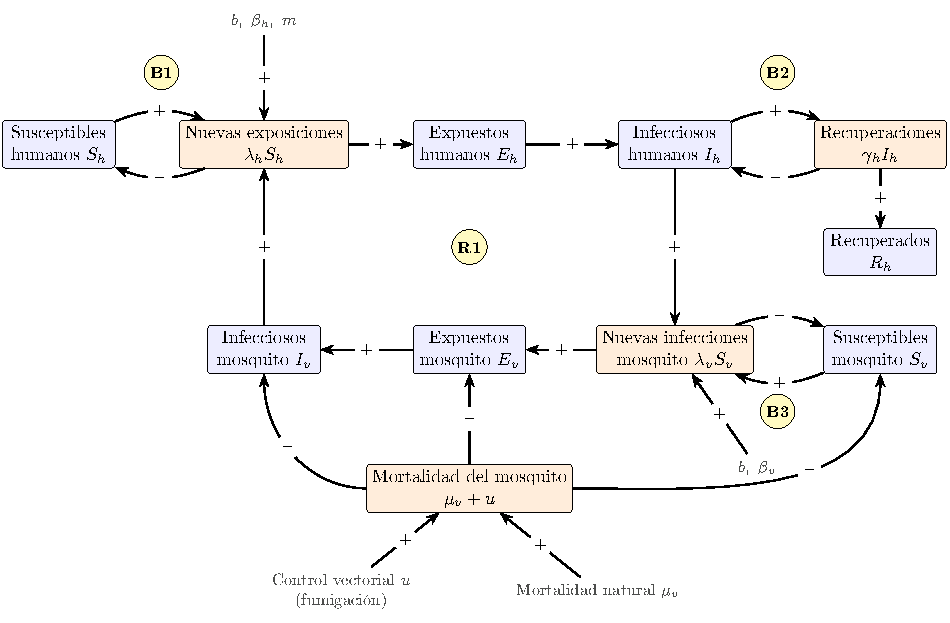
\includegraphics[width=\linewidth]{diagrama_causal_original.pdf}
\caption{Diagrama causal original. Azul: variables de estado; naranja: flujos o tasas; gris: parámetros. R1: bucle reforzador de transmisión. B1, B2 y B3: bucles compensadores por agotamiento de susceptibles humanos, recuperación y agotamiento de susceptibles vectoriales. La mortalidad actúa sobre el vector.}
\label{fig:causal}
\end{figure}

\subsection{Niveles y flujos}
En humanos, las nuevas exposiciones ocurren a una tasa $\lambda_h S_h$; los expuestos pasan a infecciosos a una tasa $\sigma_hE_h$ y los infecciosos se recuperan a una tasa $\gamma_hI_h$. Los nacimientos entran a $S_h$ y cada nivel pierde individuos por mortalidad natural.

En mosquitos, las nuevas infecciones ocurren a una tasa $\lambda_vS_v$ y la progresión a infecciosos tiene tasa $\sigma_vE_v$. El reclutamiento es constante e igual a $\mu_v$ en la escala basal. Cada nivel vectorial tiene una pérdida por mortalidad natural y por control, con tasa total $\mu_v+u$.

\begin{figure}[!htbp]
\centering
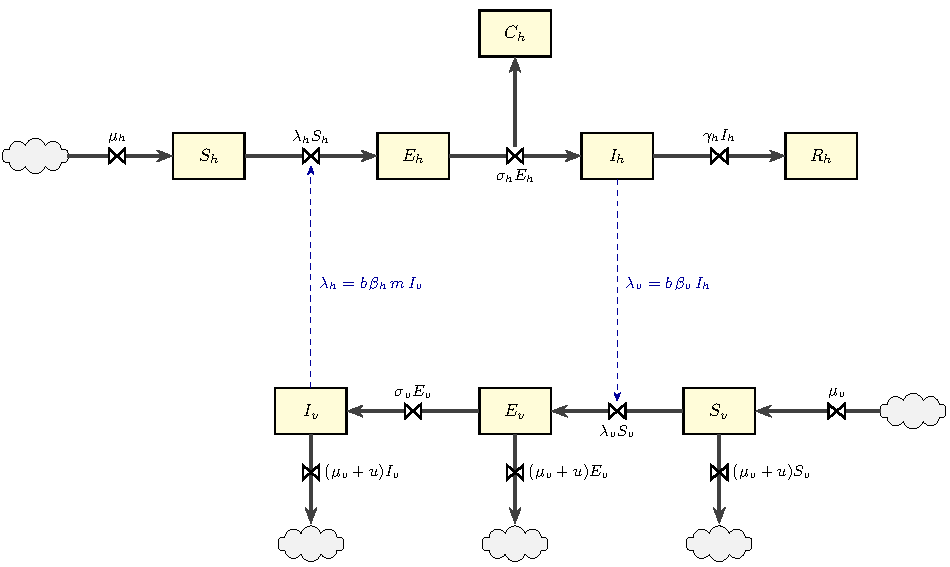
\includegraphics[width=\linewidth]{diagrama_forrester_original.pdf}
\caption{Diagrama de Forrester original. Rectángulos: niveles; flechas gruesas con válvula: flujos; nubes: fuentes y sumideros; líneas punteadas: vínculos de información. $C_h$ acumula el flujo $\sigma_hE_h$. Las muertes naturales humanas salen de cada nivel y se omiten del dibujo.}
\label{fig:dinamico}
\end{figure}

El contador $C_h$ registra la transición $E_h\to I_h$ sin alterar el balance humano. Al iniciar en cero, excluye los infecciosos presentes al comienzo.

\subsection{Ecuaciones diferenciales}
Las fuerzas de infección hacia humanos y mosquitos son
\begin{equation}
\lambda_h=b\beta_hmI_v,\qquad \lambda_v=b\beta_vI_h.
\end{equation}
El sistema humano satisface
\begin{align}
\frac{dS_h}{dt}&=\mu_h-\lambda_hS_h-\mu_hS_h,\\
\frac{dE_h}{dt}&=\lambda_hS_h-(\sigma_h+\mu_h)E_h,\\
\frac{dI_h}{dt}&=\sigma_hE_h-(\gamma_h+\mu_h)I_h,\\
\frac{dR_h}{dt}&=\gamma_hI_h-\mu_hR_h,\\
\frac{dC_h}{dt}&=\sigma_hE_h.
\end{align}
Para el vector se obtiene
\begin{align}
\frac{dS_v}{dt}&=\mu_v-\lambda_vS_v-(\mu_v+u)S_v,\\
\frac{dE_v}{dt}&=\lambda_vS_v-(\sigma_v+\mu_v+u)E_v,\\
\frac{dI_v}{dt}&=\sigma_vE_v-(\mu_v+u)I_v.
\end{align}
La suma de los niveles humanos permanece en uno. Si $N_v=S_v+E_v+I_v$, entonces
\begin{equation}
\frac{dN_v}{dt}=\mu_v-(\mu_v+u)N_v.
\end{equation}
Sin control, la población vectorial conserva su valor basal inicial. Con $u>0$, tiende a $\mu_v/(\mu_v+u)$.

\subsection{Valores iniciales y parámetros}
Se considera una introducción de 10 infecciosos por cada 10\,000 humanos en una población sin inmunidad previa. Las condiciones iniciales son supuestos del escenario y se recogen en la tabla~\ref{tab:iniciales}.
\begin{table}[!htbp]\centering
\caption{Valores iniciales de los niveles.}\label{tab:iniciales}
\begin{tabular}{lc}\toprule
Nivel & Valor inicial\\\midrule
$S_h$ & 0.999\\
$I_h$ & 0.001\\
$S_v$ & 1\\
$E_h$, $R_h$, $C_h$, $E_v$, $I_v$ & 0\\\bottomrule
\end{tabular}
\end{table}

La tabla~\ref{tab:parametros} especifica los nueve parámetros inciertos. La mortalidad humana se mantiene fija en $\mu_h=0.0000391\,\mathrm{d}^{-1}$, aproximadamente $1/(70\cdot365)$.
\begin{table}[!htbp]\centering
\caption{Parámetros nominales y rangos de exploración. Las tasas se expresan en días inversos; $\beta_h$, $\beta_v$ y $m$ son adimensionales.}\label{tab:parametros}
\small
\begin{tabularx}{\linewidth}{lXrrr}\toprule
Parámetro & Descripción & Mínimo & Nominal & Máximo\\\midrule
$b$ & Picaduras por mosquito por día & 0.3 & 0.6 & 1.0\\
$\beta_h$ & Transmisión mosquito a humano & 0.1 & 0.4 & 0.75\\
$\beta_v$ & Transmisión humano a mosquito & 0.5 & 0.7 & 1.0\\
$\sigma_h$ & Progresión humana a infeccioso & 0.10 & 0.1667 & 0.25\\
$\gamma_h$ & Recuperación humana & 0.0714 & 0.2 & 0.3333\\
$\sigma_v$ & Progresión vectorial a infeccioso & 0.0667 & 0.1 & 0.1538\\
$\mu_v$ & Mortalidad natural del mosquito & 0.033 & 0.0714 & 0.288\\
$m$ & Mosquitos basales por humano & 1 & 3 & 5\\
$u$ & Mortalidad adicional por control & 0 & 0.05 & 0.15\\\bottomrule
\end{tabularx}
\end{table}

La revisión de Andraud y colaboradores reúne enfoques de modelado del dengue \cite{andraud}. Los trabajos de Chan y Johansson y de Brady y colaboradores estudian, respectivamente, la incubación y la supervivencia del vector \cite{chan,brady}. Marini y colaboradores analizan la fumigación de ultra bajo volumen \cite{marini}. Estas referencias constituyen antecedentes biológicos y de modelado. El cotejo bibliográfico de cada extremo numérico permanece pendiente; los límites de la tabla se mantienen como supuestos explícitos del análisis, sin atribuirles una validación local. Las distribuciones uniformes se asignan a las tasas, por lo que las duraciones recíprocas no tienen distribución uniforme.

\subsection{Número reproductivo en el equilibrio con control}
En ausencia de infección, el equilibrio vectorial es $S_v^*=\mu_v/(\mu_v+u)$. El número reproductivo para ese equilibrio cumple
\begin{equation}\label{eq:r0}
R_0^2=
\frac{b^2\beta_h\beta_vm\sigma_h\sigma_v\mu_v}
{(\gamma_h+\mu_h)(\sigma_h+\mu_h)(\mu_v+u)^2(\sigma_v+\mu_v+u)}.
\end{equation}
La raíz cuadrada corresponde a la convención que considera las generaciones humana y vectorial. La tasa de picadura aparece al cuadrado porque participa en ambos sentidos de transmisión. Con los parámetros nominales se obtiene $R_0\approx1.82$.

El umbral $R_0=1$ corresponde al equilibrio con control. La simulación comienza con $S_v(0)=1$, por lo que atraviesa un ajuste de la densidad vectorial antes de acercarse a ese equilibrio. Esta diferencia debe tenerse en cuenta al interpretar el crecimiento inicial.

\section{Solución numérica y verificación}
El sistema se integra en el intervalo de 0 a 365 días mediante Runge-Kutta de cuarto orden, con paso fijo de 0.05 días. El programa del curso traduce el modelo a C y ejecuta las simulaciones. La comprobación independiente utiliza LSODA en Python, con tolerancia relativa $10^{-9}$ y absoluta $10^{-12}$ para las 999 combinaciones de parámetros.

En el escenario nominal, el pico de $I_h$ es aproximadamente el 6.65\,\% de la población alrededor del día 112. La fracción máxima de mosquitos infecciosos es aproximadamente el 4.8\,\% de su población basal. El acumulado $C_h(365)$ es aproximadamente 0.9336.

La diferencia máxima absoluta entre las salidas del programa del curso y LSODA es cercana a $5\times10^{-7}$ en $I_h$ e $I_v$ y a $5\times10^{-6}$ en $C_h$. Estos valores corresponden al orden de precisión de los archivos exportados. La comprobación también evalúa la conservación humana, el balance vectorial, la no negatividad y la acumulación monótona de $C_h$.

$C_h(365)$ expresa las entradas acumuladas a la clase infecciosa por unidad de población de referencia. Puede superar uno por la renovación demográfica. Su interpretación como probabilidad individual o como tamaño final requiere precaución: algunas corridas todavía crecen al terminar el horizonte.

\section{Análisis de incertidumbre y sensibilidad}
\subsection{Diseño LHS y variables de salida}
Se muestrean nueve parámetros mediante hipercubo latino con 999 muestras y semilla 20261118. Cada parámetro tiene una distribución uniforme dentro del rango declarado. El análisis en Python reutiliza la matriz de parámetros del programa del curso.

Las salidas temporales son $I_h(t)$, $I_v(t)$ y $C_h(t)$. Las salidas escalares son $C_h(365)$, el máximo de $I_h$, el día en que se alcanza y $R_0$. El máximo y su día se evalúan en una malla diaria en Python.

Para analizar el día del pico se exige que el máximo supere $2I_h(0)$ y ocurra en un día interior al intervalo. El criterio selecciona 569 corridas. Otras 35 alcanzan su máximo observado al día 365, de modo que su pico completo queda sin determinar dentro del horizonte.

\subsection{Cálculo e interpretación del PRCC}
El PRCC cuantifica la relación entre un parámetro y una salida después de transformar los datos a rangos y controlar linealmente el efecto de los demás parámetros en esa escala \cite{marino}. Un coeficiente positivo indica una asociación creciente y uno negativo una asociación decreciente. La interpretación depende de la monotonía de la relación y de los rangos asignados.

Los valores $p$ se calculan con la aproximación basada en la distribución $t$ de Student. Los asteriscos de las figuras corresponden a $p<0.05$, sin ajuste por comparaciones múltiples. La significancia estadística se interpreta junto con la magnitud del coeficiente y las limitaciones del modelo.

En las salidas temporales pueden aparecer cruces de trayectorias. Una transmisión más rápida puede elevar la prevalencia al inicio y reducirla después porque el brote se adelantó. Por ello, un PRCC tardío próximo a cero no basta para concluir que un parámetro tiene poca influencia. La ejecución conserva gráficos de dispersión por rangos para los nueve parámetros frente a las salidas escalares y frente a $I_h$ en los días 60, 120 y 240. Estos gráficos permiten examinar el supuesto de monotonía; su generación por sí sola no lo certifica.

\subsection{Incertidumbre de las trayectorias}
La mediana de $R_0$ es 1.25 y sus percentiles 5 y 95 son 0.43 y 3.61. El 62.9\,\% de las muestras tiene $R_0>1$. La mediana de $C_h(365)$ es el 57.7\,\% de la población de referencia. Las bandas de la figura~\ref{fig:incertidumbre} describen la variación entre los escenarios muestreados.
\grafico{fig1_trayectorias.png}{1}{Trayectorias humanas y vectoriales: mediana y bandas de percentiles de 999 corridas LHS. Los mosquitos se expresan respecto de la población basal.}{fig:incertidumbre}

\subsection{Sensibilidad de las salidas}
La figura~\ref{fig:prcctiempo} muestra el PRCC temporal, y la figura~\ref{fig:prccescalar} resume los coeficientes del acumulado, el pico y su día. Los valores escalares se recogen en la tabla~\ref{tab:prcc}.
\grafico{fig2_prcc_tiempo.png}{1}{PRCC frente a la prevalencia humana, los mosquitos infecciosos y los casos acumulados. Los puntos indican valores $p<0.05$ sin ajuste múltiple.}{fig:prcctiempo}
\grafico{fig3_prcc_outcomes.png}{1}{PRCC de las salidas escalares. El día del pico se analiza en 569 corridas con un máximo interior superior a dos veces la prevalencia inicial.}{fig:prccescalar}
\begin{table}[!htbp]\centering
\caption{PRCC frente a las salidas escalares. Los valores se redondean a dos decimales; el CSV adjunto conserva los valores $p$ y una mayor precisión.}\label{tab:prcc}
\setlength{\tabcolsep}{3pt}\footnotesize
\begin{tabular}{lrrrrrrrrr}\toprule
Salida ($n$) & $b$ & $\beta_h$ & $\beta_v$ & $\sigma_h$ & $\gamma_h$ & $\sigma_v$ & $\mu_v$ & $m$ & $u$\\\midrule
$C_h(365)$ (999) & +0.87 & +0.81 & +0.41 & +0.00 & -0.72 & +0.37 & -0.71 & +0.74 & -0.82\\
Pico (999) & +0.74 & +0.62 & +0.25 & +0.06 & -0.69 & +0.26 & -0.42 & +0.56 & -0.65\\
Día del pico (569) & -0.80 & -0.73 & -0.46 & -0.20 & +0.51 & -0.36 & +0.57 & -0.70 & +0.75\\
$R_0$ (999) & +0.88 & +0.81 & +0.43 & +0.00 & -0.74 & +0.37 & -0.70 & +0.74 & -0.83\\
\bottomrule\end{tabular}\end{table}


El acumulado presenta las asociaciones positivas más altas con $b$ (0.87), $\beta_h$ (0.81) y $m$ (0.74). El control $u$ tiene un coeficiente de aproximadamente $-0.82$; la recuperación humana y la mortalidad natural del mosquito presentan coeficientes cercanos a $-0.72$ y $-0.71$. Dentro de los rangos elegidos, una mayor transmisión favorece la acumulación de infecciones, mientras una recuperación más rápida y una menor supervivencia vectorial la reducen.

La tasa de progresión humana $\sigma_h$ tiene un PRCC cercano a cero para el acumulado. En cambio, aparece una asociación negativa con el día del pico. La incubación vectorial interviene también en la probabilidad de sobrevivir hasta ser infeccioso, lo que explica su relación con la transmisión.

En las 569 corridas seleccionadas, mayores valores de $b$, $\beta_h$ y $m$ se asocian con un pico más temprano. El control y la mortalidad vectorial se asocian con un pico más tardío. La selección depende de la presencia y localización del pico, de modo que estos coeficientes describen ese subconjunto y no deben extrapolarse a todas las simulaciones.

\section{Comparación de escenarios de control}
Se comparan $u=0$, $u=0.05$ y $u=0.15\,\mathrm{d}^{-1}$ manteniendo los demás parámetros en sus valores nominales. La tabla~\ref{tab:control} y la figura~\ref{fig:control} presentan las diferencias.
\begin{table}[!htbp]\centering
\caption{Resultados de los escenarios de control. El día del máximo se evalúa en una malla diaria.}\label{tab:control}
\begin{tabular}{rrrr}\toprule
$u$ ($\mathrm{d}^{-1}$) & Máximo de $I_h$ (\%) & Día del máximo & $C_h(365)$\\\midrule
0 & 14.49 & 67 & 1.0011\\
0.05 & 6.65 & 112 & 0.9336\\
0.15 & 0.10 & 0 & 0.00451\\\bottomrule
\end{tabular}
\end{table}
\grafico{controles.png}{1}{Comparación controlada de la prevalencia humana y el acumulado para tres valores de mortalidad adicional. Los demás parámetros permanecen fijos.}{fig:control}

Con $u=0.05$, el pico es menor y ocurre más tarde que en ausencia de control. Con $u=0.15$, el máximo corresponde a la condición inicial y no aparece un pico epidémico interior. En estos escenarios, el control reduce la transmisión y puede evitar el crecimiento epidémico; el retraso del pico solo tiene sentido cuando existe un pico interior.

\section{Verificación del cálculo de sensibilidad}
El ejecutable \texttt{prcc\_fix} reinicia la variable de agrupación de empates antes de calcular los rangos en cada instante. Esta corrección evita que los grupos de un instante afecten al siguiente. El programa original se conserva para comparación.

Sobre las mismas trayectorias redondeadas, la diferencia máxima entre el PRCC corregido y el cálculo Python es menor de $5\times10^{-7}$. La comparación con trayectorias independientes de LSODA alcanza diferencias cercanas a 0.005 en prevalencias, debidas al efecto del redondeo sobre los rangos.

En la ejecución comparativa, la diferencia máxima entre el programa original y el corregido es 0.004239 para $I_h$, 0.017534 para $I_v$ y 0.127563 para $C_h$. Estos valores corresponden a esa ejecución del programa original y no garantizan que su comportamiento sea determinista.

\clearpage
\section{Discusión y conclusiones}
El análisis identifica a la picadura, la transmisión al humano y la densidad vectorial como parámetros con asociaciones positivas altas frente al acumulado. La mortalidad adicional por control, la recuperación humana y la mortalidad natural del mosquito presentan asociaciones negativas altas. El orden y la magnitud de estas asociaciones dependen de los rangos utilizados.

El modelo supone mezcla homogénea, un solo serotipo e inmunidad tras la recuperación. No incorpora estacionalidad, clases asintomáticas ni estructura espacial. El control se mantiene constante durante todo el periodo. Los valores iniciales y los límites paramétricos representan decisiones de modelado, y la falta de calibración limita la aplicación a una población concreta.

La comparación independiente respalda la solución numérica y el cálculo de sensibilidad sobre los datos simulados. La validación epidemiológica requeriría contrastar las trayectorias con datos observados. Bajo los supuestos actuales, el control reduce la transmisión en los escenarios comparados; cuando es suficientemente alto, desaparece el pico epidémico interior.

\clearpage
\addcontentsline{toc}{section}{Referencias}
\bibliographystyle{unsrt}
\bibliography{referencias}

\clearpage
\section*{Reproducción del análisis}
\markright{Reproducción del análisis}
\addcontentsline{toc}{section}{Reproducción del análisis}
Los datos del informe proceden de la ejecución \texttt{work/mejora\_20261120}. La carpeta \texttt{datos} contiene el CSV de coeficientes y los metadatos; las figuras utilizadas se incluyen junto a las fuentes LaTeX.

Desde la raíz del repositorio, se prepara una carpeta nueva para conservar los resultados anteriores:
\begin{lstlisting}[language=bash]
docker build -t lhsprcc .
mkdir -p work
mkdir work/ejecucion_nueva
cp models/dengue.txt models/ejemplo_sir.txt \
   scripts/analisis_prcc.py work/ejecucion_nueva/
docker run --rm -it -v "$PWD/work:/work" lhsprcc
\end{lstlisting}
Dentro del contenedor:
\begin{lstlisting}[language=bash]
cd /work/ejecucion_nueva
lhsrun ejemplo_sir.txt
lhsrun dengue.txt
python3 analisis_prcc.py out_dengue figuras
\end{lstlisting}
Para generar los diagnósticos desde la raíz del repositorio, con NumPy, SciPy y Matplotlib disponibles:
\begin{lstlisting}[language=bash]
python3 scripts/diagnosticos_dengue.py \
  work/ejecucion_nueva/out_dengue \
  work/ejecucion_nueva/diagnosticos
\end{lstlisting}
La carpeta de diagnósticos debe ser nueva. Para reproducir exactamente las tablas de este informe se utiliza la matriz LHS conservada en la ejecución indicada y el CSV incluido.
\end{document}
